\documentclass[12pt]{report}
\usepackage[utf8]{inputenc}
\usepackage{geometry}
\usepackage{hyperref}
\usepackage{multicol}
\usepackage{graphicx}
\usepackage{listings}
\usepackage{xcolor}
\usepackage{color}

\geometry{bottom=30mm, top=30mm, left=30mm, right=30mm}

\newcommand{\deadline}[3]{
    \hspace{0pt}
    \vfill
    \begin{center}
        \Huge \textbf{Deadline #1} \\
        \vspace*{5pt}
        \Large \textit{#2} \\
        \vspace*{25pt}
        \large \textbf{#3}
    \end{center}
    \vfill
    \pagebreak
}

\definecolor{dkgreen}{rgb}{0, 0.6, 0.0}
\definecolor{gray}{rgb}{0.5, 0.5, 0.5}
\definecolor{mauve}{rgb}{0.58, 0.0, 0.82}

\lstset{frame=tb,
    language=SQL,
    aboveskip=3mm,
    belowskip=3mm,
    showstringspaces=false,
    columns=flexible,
    basicstyle={\small\ttfamily},
    numbers=none,
    numberstyle=\tiny\color{gray},
    keywordstyle=\color{blue},
    commentstyle=\color{dkgreen},
    stringstyle=\color{mauve},
    breaklines=true,
    breakatwhitespace=true,
    tabsize=4
}

\title{
    \textbf{\Huge ElectroBase Management System} \\
    \vspace*{15pt}
    \large{
        EBMS - \textit{an Online Electronics Retail Store}, built as a course project for
        \normalsize{CSE202: Fundamentals of Database Management Systems} \\
    }
    \vspace*{20pt}
    \textbf{\Large Project Report and Documentation}
}

\author{
    \href{mailto:divyajeet21529@iiitd.ac.in}{]Divyajeet Singh (2021529)}
    \and
    \href{mailto:mehar21541@iiitd.ac.in}{Mehar Khurana (2021541)}
}

\date{\vspace*{10pt} \textbf{\today}}

\begin{document}
    \maketitle

    \deadline{1}{Defining Project Scope and Requirements}{January 25, 2023}

    \section*{\Huge Project Scope}
    \vspace*{10pt}
    Electronics has always been a booming industry.
    With the advent of the internet, the industry has seen a massive shift towards online retail.
    However, it is difficult to keep track of the technical requirements of a store.
    It is difficult to keep all stakeholders in the loop and keep them involved and updated.
    \vspace*{10pt} \\
    This is where we come in with \textbf{EBMS}, i.e. the \textbf{ElectroBase Management System}.
    EBMS is an online retail platform for electronics.
    It aims to provide a common platform for suppliers, store managers, customers, and delivery agents.
    \begin{itemize}
        \item
        It is an easy solution for the \textbf{customers}, as it aims to provide a diverse catalogue of products to customers.
        The customers get to choose from a wide range of categories, make changes to their cart, and make secure payments with a method of their choice.
        \item
        The \textbf{suppliers} get to keep track of their products and change their description, price, etc.
        They can also keep track of their sales statistics and make changes to their products as and when required.
        \item
        The database managers (\textbf{admins}) get assisted in monitoring the transactions and managing the inventory.
        Based on their requirements, they can add deals or combos on the available products or remove categories from their store.
        \item
        EBMS provides a platform for \textbf{delivery agents} to keep track of all orders that have been assigned to them. They can set their activity/inactivity status and view the feedback given to them.
    \end{itemize}
    The primary focus of the project is to design an efficient backend.
    We aim to create a system that is smooth and easy to use for the customers and easy to manage for the suppliers.
    The system should support efficient searching through the catalogue and should be able to handle a large number of transactions.
    \vspace*{10pt} \\
    The backend will be built using MySQL, along with Python and Django, and will be hosted on a server.
    The frontend will be built using HTML, CSS, and ReactJS.
    By the end of the semester, we plan to host this project on a public server and make it accessible publicly.

    \subsection*{TL; DR}
    The aim of this project is to bring to life an integrated online retail store for electronics.
    The project will bring all stakeholders on a common platform and will ensure a smooth and easy-to-use experience for the customers.

    \section*{\Huge Technical Requirements}
    \subsection*{Tech Stack}
    We plan for EBMS to be a full-stack project with a backend and a frontend.
    According to the requirements, we plan to use the following tools and technologies:
    \textbf{\begin{multicols}{2}
        \begin{itemize}
            \item MySQL Database
            \item Python-3
            \item Django Framework
            \item HTML
            \item CSS
            \item ReactJS
        \end{itemize}
    \end{multicols}}

    \subsection*{Entities, Relations, \& Constraints}

    \subsubsection*{Entities}
        The following entities are identified and will be used in the project:
        \begin{enumerate}
            \item \textbf{Admin:}
            Admins are the store managers.
            They are the stakeholders responsible for managing the inventory and maintaining the store (database).
            \item \textbf{Customers:}
            Customers are the primary stakeholders interacting with the system.
            They must create an account and log in to use the app.
            \item \textbf{Suppliers:}
            Suppliers are responsible for supplying products to the store.
            Different suppliers are allowed to supply the same products to the store.
            \item \textbf{Delivery Agents:}
            A delivery agent will be assigned to each order.
            They will be responsible for delivering orders.
            \item \textbf{Products:}
            As the name suggests, these are the products supplied to the store by suppliers.
            Products are weak entities since several sellers can sell the same product, ie, we can have several records for the same productID.
            \item \textbf{Orders:}
            An order entity is used to keep track of the orders placed by different customers.
            Each order also has one associated delivery agent.
            \item \textbf{Product Reviews:}
            Product reviews are the feedback given by customers on products.
            A customer can only review a product they have previously purchased.
            \item \textbf{Delivery Agent Reviews:}
            Delivery agent reviews are the feedback given by customers to delivery agents.
            A customer can only post a review on a delivery agent they have received an order from.
            \item \textbf{Wallet:}
            A wallet is a belonging of a customer that stores attributes like the current balance of the customer, their UPI-ID etc.
            Users' wallets are hidden from the admin's view. Wallets are weak entities since several people can be using the same UPI-ID, and we require the customerID to uniquely identify a wallet.
            \item \textbf{Description:}
            The description weak entity is used to store the description of different products.
            This is used to avoid redundancy of data storage (in the case where multiple suppliers are selling the same products with the same descriptions).
        \end{enumerate}

    \subsubsection*{Relationships \& Cardinality Constraints}
    To effectively manage the database, we will be using the following (non-exhaustive list of) relationships among the data:
    \begin{enumerate}
        \item \textbf{\textit{Cart}:}
        Cart is a relationship between \textbf{Customer} and \textbf{Product}.
        One customer can add multiple products to the cart (and choose a specific supplier).
        The same products may be added to more than one cart. When a customer checks out, the cart is used to generate an order entity, and a delivery agent is assigned to it.
        \item \textbf{\textit{Sells}:}
        \textbf{Supplier} \textit{sells} \textbf{Product}.
        This many-to-many relationship is used to keep track of what products one supplier sells.
        Each supplier can supply multiple products. The same product may be sold by different suppliers.
        \item \textbf{\textit{Sold}:}
        \textbf{Supplier} has \textit{sold} \textbf{Product}.
        This many-to-many relationship covers the products sold by a supplier and will be used to generate their sales statistics.
        \item \textbf{\textit{Delivered}:}
        \textbf{Delivery Agent} has \textit{delivered} to \textbf{Customer}.
        This is a ternary relationship involving \textbf{Delivery Agent Review} as well.
        There can be, at most, one (editable) review from one customer for a delivery agent.
        \item \textbf{\textit{Purchased}:}
        \textbf{Customer} has \textit{purchased} \textbf{Product}.
        This is a ternary relationship involving \textbf{Product Review} as well.
        There can be, at most, one (editable) review from one customer for a product.
        \item \textbf{\textit{Describes}:}
        \textbf{Description} \textit{describes} \textbf{Product}.
        This is a one-to-one relationship.
        \item \textbf{\textit{Belongs To}:}
        \textbf{Wallet} \textit{belongs to} \textbf{Customer}.
        This is a one-to-one relationship.
        \item \textbf{\textit{Consists Of}:}
        \textbf{Order} \textit{consists} \textbf{Products}.
        This is a one-to-many relationship, as one order may consist of multiple products. The product quantities are moved from the cart to the order on checkout.
        \item \textbf{\textit{Manages}:}
        \textbf{Admin} \textit{manages} the app.
        This relationship is used to hide entities like wallets from the admin's view.
    \end{enumerate}
    Most cardinality constraints have been mentioned above in the description of relationships.
    Some other constraints are as follows:
    \begin{enumerate}
        \item \textbf{Existential:}
        \begin{enumerate}
            \item \textbf{Product - Supplier:} There can be no product without a supplier.
            \item \textbf{Order - Customer:} An order cannot exist without a customer.
            \item \textbf{Order - Delivery Agent:} An order cannot exist without a delivery agent.
            \item \textbf{Product Review - Customer \textit{has purchased} Product:} To ensure that a customer can review only the products they have purchased.
            \item \textbf{Delivery Agent Review - Delivery Agent \textit{delivered to} Customer:} to ensure that a customer can review only the delivery agents they have received orders from.
        \end{enumerate}
        \item \textbf{One-to-One:}
        \textbf{Delivery Agent - Order:} One delivery agent can be assigned at most one order at a time.
        We may remove this constraint later and implement an algorithm to find the best agent to assign an order to, based on the current delivery addresses, with a cap on the number of orders per agent.
        \item \textbf{One-to-Many:}
        \textbf{Customer - Phone Number} One customer can have multiple phone numbers.
        It will be implemented as a multi-valued attribute of Customer.
    \end{enumerate}

    \subsubsection*{Access Constraints}
    Since some data must remain private while other data must be accessible to all, the following access-control constraints will be implemented:
    \begin{enumerate}
        \item \textbf{Admin:} All data except for Customer passwords and Wallets
        \item \textbf{Customer:} Personal records, past and current Orders, and all Products and Reviews
        \item \textbf{Supplier:} Their Product catalogue, personal records, sales statistics, and Customer Reviews
        \item \textbf{Delivery Agent:} Personal records, current Orders, and Reviews from past Orders
    \end{enumerate}

    \section*{\Huge Functional Requirements}
    \vspace*{10pt}
    All stakeholders except the \textbf{Admins} will need to create an account and log in.
    The following (non-exhaustive list of) features are some of the functional requirements of the project:
    \begin{enumerate}
        \item As a \textbf{Customer:}
        \begin{itemize}
            \item Add balance to wallet
            \item Browse and search/sort/filter for products
            \item Manage (add/remove) items in their cart
            \item Place an order (checkout cart)
            \item Confirm/Authenticate transaction
            \item View and search for previous orders
        \end{itemize}

        \item As an \textbf{Admin:}
        \begin{itemize}
            \item Add/Delete categories
            \item Delete products
            \item Add/Modify discounts
            \item Create deals/combos
            \item View transaction history
            \item Appoint other Admins
        \end{itemize}

        \item As a \textbf{Supplier:}
        \begin{itemize}
            \item View products currently on sale
            \item Add/Discontinue a product
            \item Change price of a product
            \item Change quantity of a product
            \item View sales statistics
        \end{itemize}

        \item As a \textbf{Delivery Agent:}
        \begin{itemize}
            \item Confirm a delivery
            \item View the address of the order
            \item View the ETA of the order
            \item View reviews
            \item Choose current activity status
        \end{itemize}
    \end{enumerate}

    \pagebreak

    \deadline{2}{Designing the ER Model and converting it to a Relational Model}{February 3, 2023}

    \section*{\Huge Entity-Relationship Model}
    \vspace*{10pt}
    Entity-Relationship (ER) Models are used to plan how different entities in a project interact with each other. \\
    \newline
    Our ER Model captures the nature of the relationships and entities planned to be used in the project.
    The ER Model is designed in accordance with the assumptions and constraints as mentioned in the document above.
    Hence, we plan to build our system on the basis of the following Entity-Relationship Model:
    \vspace*{10pt}
    \begin{center}
        \hspace*{-37pt}
        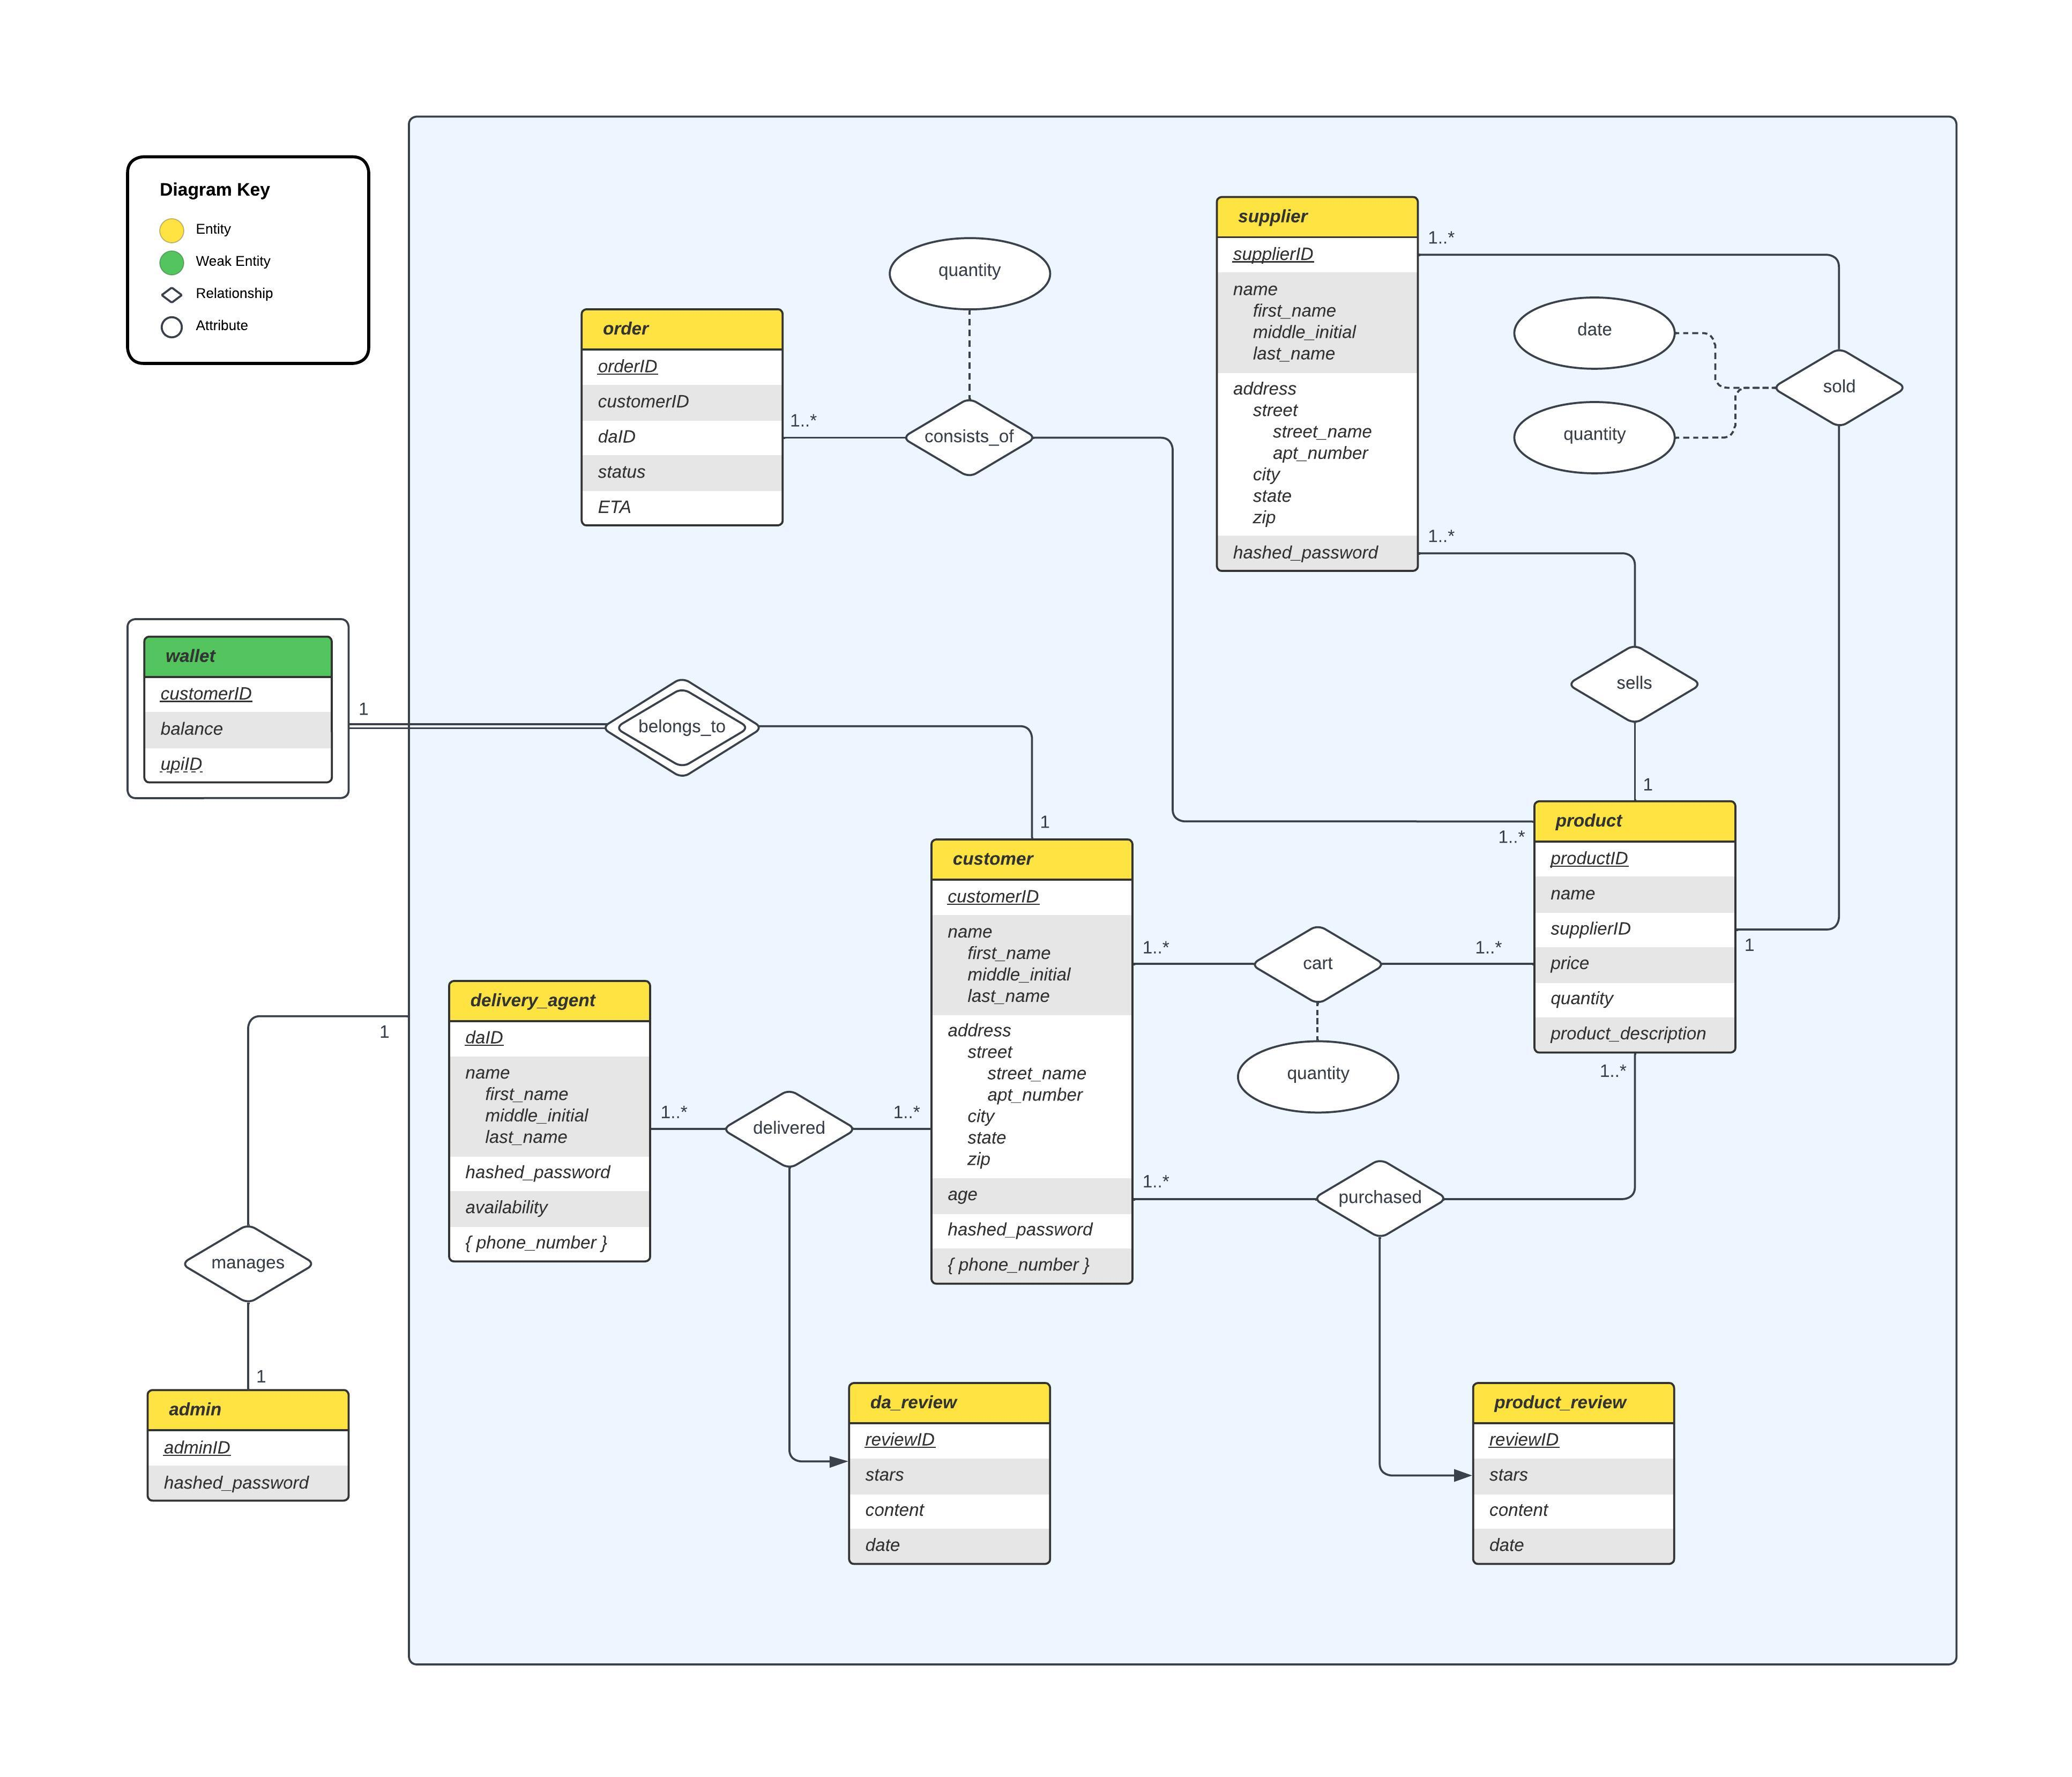
\includegraphics[scale=0.6]{Assets/ER-Model}
    \end{center}

    \subsection*{Ternary Relationships}
    The following ternary relationships have been identified:
    \begin{enumerate}
        \item \textbf{Customer - Product - Product Review:}
        A customer can review multiple products, and a product can be reviewed by multiple customers.
        A customer can give at most one review per product.
        This ternary relationship will be decomposed into the following binary relationships at the time of implentation:
        \begin{enumerate}
            \item \textbf{Customer - Product:}
            (Many-to-Many) To keep track of which customers have purchased which products.
            \item \textbf{Product - Product Review:}
            (One-to-Many) To keep track of all reviews given to a product.
            \item \textbf{Customer - Product Review:}
            (One-to-Many) To keep track of all reviews given by a customer.
            This relationship may not be needed and may be removed in the future.
        \end{enumerate}
        \item \textbf{Delivery Agent - Customer - Delivery Agent Review:}
        A customer can review multiple delivery agents, and a delivery agent can be reviewed by multiple customers.
        A customer can give at most one review per delivery agent.
        This ternary relationship will be decomposed into the following binary relationships at the time of implentation:
        \begin{enumerate}
            \item \textbf{Customer - Delivery Agent:}
            (Many-to-Many) To keep track of which customers have received orders from which delivery agents.
            \item \textbf{Delivery Agent - Delivery Agent Review:}
            (One-to-Many) To keep track of all reviews given to a delivery agent.
            \item \textbf{Customer - Delivery Agent Review:}
            (One-to-Many) To keep track of all reviews given by a customer.
            This relationship may not be needed and may be removed in the future.
        \end{enumerate}
    \end{enumerate}

    \section*{\Huge Relational Model}
    \vspace*{10pt}
    Relationship Models are used to represent how data will be stored in the database, along with the attributes of each entity and relationship.
    The Relational Model is designed in accordance with the assumptions and constraints as mentioned in the document above. \\
    \newline
    \textbf{Note:} The arrows represent that a field is \textit{derived} from another.
    For example, \verb|productID| in \verb|description| will contain values of \verb|productID| from table \verb|product|.
    \pagebreak
    \vspace*{35pt}
    \begin{center}
        \hspace*{-40pt}
        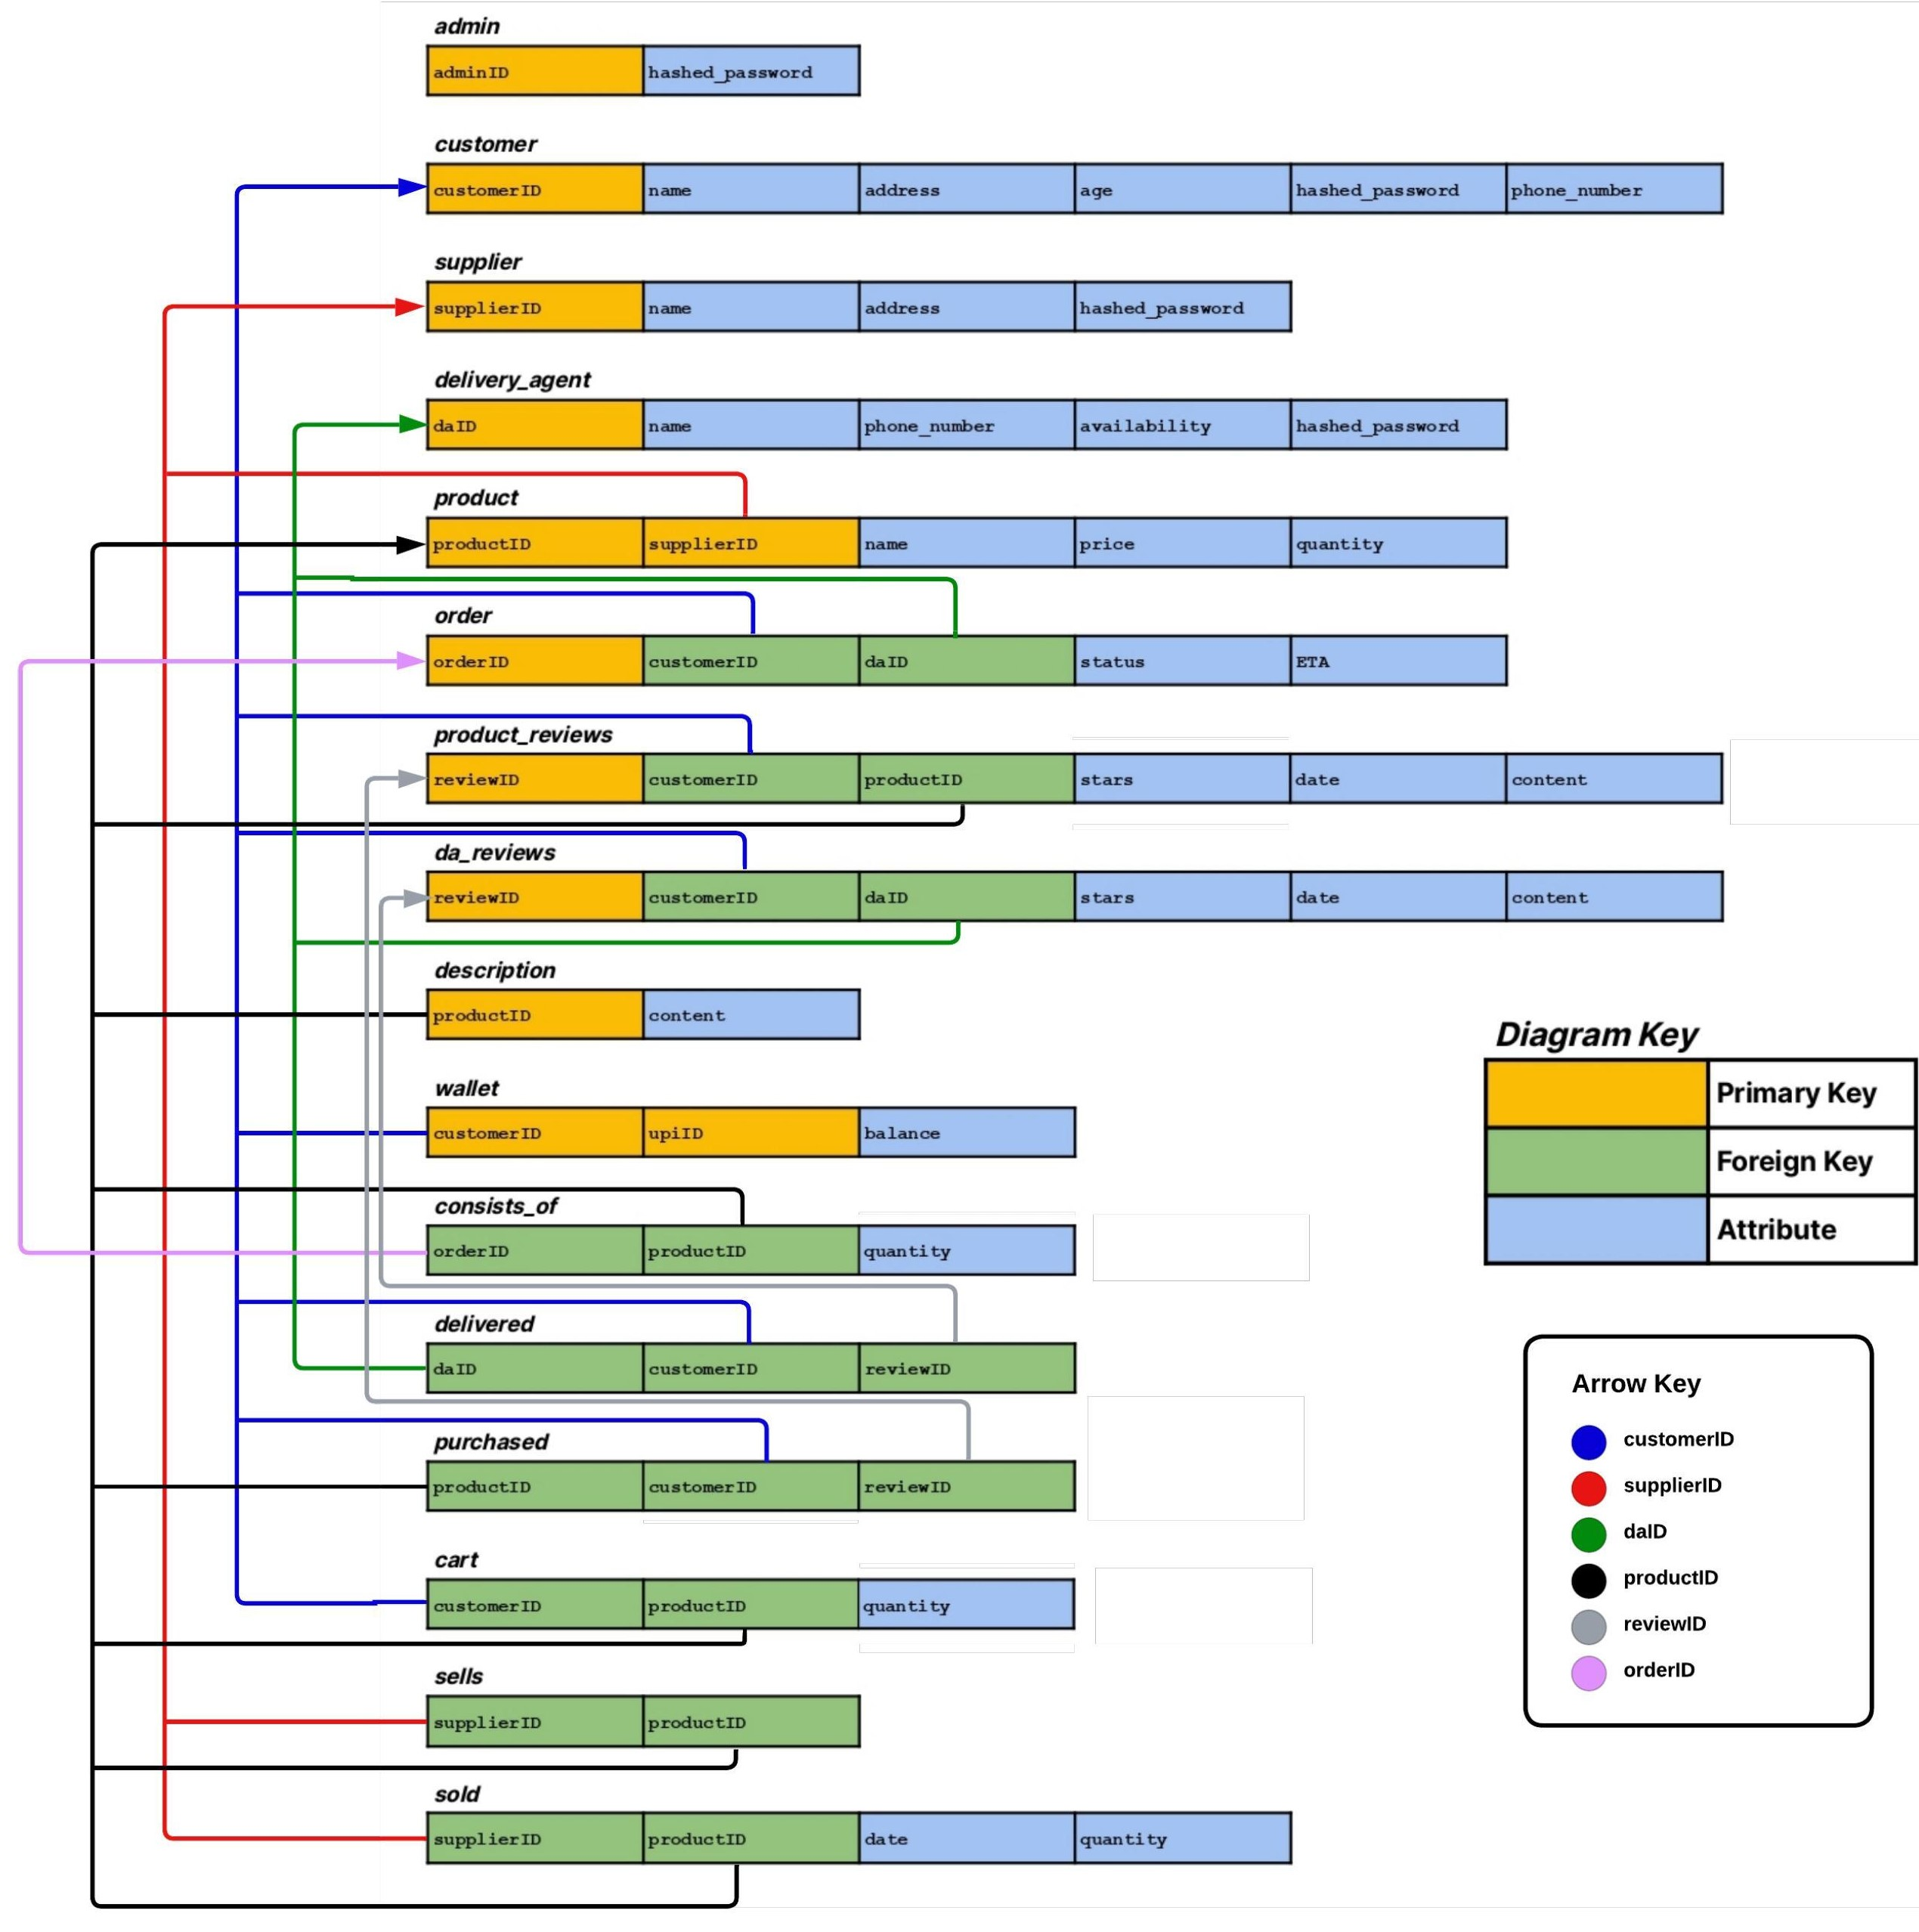
\includegraphics[scale=0.8]{Assets/Relational-Model}
    \end{center}

    \pagebreak

    \deadline{3}{Implementing the Database Schema and Integrity Constraints, and Populating simulated data satisfying them}{February 10, 2023}

    \section*{\Huge Iterations on the Database Schema}
    \subsection*{Tables added or renamed:}
    \begin{enumerate}
        \item
        Since \textbf{address} is a composite attribute, we store it in a separate table since we would rarely need to search for the address.
        The search/join/union query efficiency would get affected if we store all the address data in the same stakeholder table.
        \item
        The \textbf{consists\_of} relationship table has been renamed to \textbf{order\_product} to make it more intuitive.
        \item
        Entity table \textbf{description} has been renamed to \textbf{product\_description}, since \verb|description| is a reserved keyword in MySQL.
        Its field \textbf{description} has also been renamed to \textbf{content} for the same reason.
        \item
        Entity table \textbf{order} has also been renamed to \textbf{orders} for the same reason.
    \end{enumerate}

    \subsection*{Columns/Fields added, removed, or renamed:}
    \begin{enumerate}
        \item
        All fields called \textbf{hashed\_password} have been renamed to \textbf{pwd} for simplicity.
        \item
        Added field \textbf{email} to \textbf{customer}, \textbf{supplier}, and \textbf{delivery\_agent} tables.
        \item
        Added field \textbf{quantity} to table \textbf{product}.
        \item
        Removed fields \textbf{reviewID} from the \textbf{product\_review} and \textbf{da\_review} tables, so as to decompose the ternary relationships \textbf{delivered} and \textbf{purchased}.
        \item
        Added \textbf{order\_date} and \textbf{delivery\_date} to the \textbf{order} table.
    \end{enumerate}

    \section*{\Huge Handling Different Attributes}
    \subsection*{Composite Attributes:}
    \begin{enumerate}
        \item
        Addresses of all stakeholders are stored in a single table with a unique \textbf{addressID} assigned to each address.
        This \textbf{addressID} is then stored along with other stakeholder data in their tables.
        \item
        Added sub-attribute \textbf{country} to the \textbf{address} composite attribute.
        \item
        The \textbf{name} composite attribute is stored in the same table, since we might need to search for the names of the stakeholders.
        Each sub-attribute is kept as a column (\textbf{first\_name}, \textbf{middle\_initial}, \textbf{last\_name}) in the table.
    \end{enumerate}

    \subsection*{Multi-Valued Attributes:}
    \begin{enumerate}
        \item
        Since \textbf{phone\_number} is a multivalued attribute, we store it in a separate table, with the \textbf{phoneID} attribute from this table being stored in the \textbf{delivery\_agent} and \textbf{customer} tables.
        This table does not have a primary key since each \textbf{phoneID} associates to one or more \textbf{num}'s (phone numbers).
    \end{enumerate}

    \subsection*{Derived Attributes:}
    \begin{enumerate}
        \item
        Changed \textbf{ETA} and \textbf{delivered} (earlier \textbf{status}) to derived attributes.
        \textbf{ETA} will be calculated as \textbf{order\_date} + 15 days when required.
        \item
        The attribute \textbf{delivered} will be \verb|true| if \textbf{delivery\_date} is not null, else \verb|false|.
    \end{enumerate}
    Since these constraints/relations will be implemented outside the database, and hence these fields are not present in the tables.

    \section*{Assumptions:}
    \begin{enumerate}
        \item
        The field \textbf{delivery\_date} of \textbf{orders} is allowed to be \verb|NULL|.
        This is because we do not know the \textbf{delivery\_date} when the order is placed, and it is only updated when the order is delivered.
        We derive the attribute \textbf{delivered} from \textbf{delivery\_date} to check if the order has been delivered or not.
        \item
        Since \textbf{phone numbers} are implemented as multi-valued attributes, we assume that phone numbers are not unique to a customer.
        This means that multiple users may have the same phone number.
        \item
        All primary keys are defined with the \verb|AUTO_INCREMENT| constraints so that we do not need to insert ID values ourselves, and duplicity errors on primary keys are avoided.
        \item
        \textbf{Product descriptions} and \textbf{review contents} are being stored using \verb|TEXT| datatype in MySQL, which is not stored in the server memory and does not hamper query times.
        \item
        All attributes that can not have null values have been specified as \verb|NOT NULL|. Attributes like \textbf{last\_name}, \textbf{middle\_initial}, \textbf{content} in the \textbf{review} tables, and \textbf{delivery\_date} in the \textbf{orders} table can have null values.
        \item
        \textbf{Availability} of a delivery agent has been given a \verb|DEFAULT| value of true, ie, when a delivery agent is added to the database, he is available to deliver an order by default.
        \item
        \textbf{Balance} in a customer wallet, on account creation, has been given a \verb|DEFAULT| value of 0.
        \item
        \textbf{pwd}'s in all tables are stored as SHA1 hashes.
        \item
        Some other integrity constrains have also been added, for example, \textbf{rating} must be between 0 and 5, and \textbf{quantity} and \textbf{price} must be positive.
        \item
        Based on a rough idea of the types of queries we plan to use, some indices have also been added on the fields of the tables.
        These may be updated in the future.
    \end{enumerate}

    \section*{\Huge Data Generation \& Population}
    \subsection*{Data Generation}
    Most of the simulated data for the stakeholder and main entity tables was generated using \href{https://www.mockaroo.com}{\color{blue}\underline{https://www.mockaroo.com}}. \\
    \newline
    We utilised the (Ruby) code functionality to implement viable constraints on the data while data generation.
    The data for each table was downloaded as a CSV-file.
    We then used python scripts to generate the MySQL insertion queries and to populate relations.
    Data for some tables (like \textbf{cart} and \textbf{orders}) was mainly done through python scripts so as to make sure the existential constraints were not violated.

    \subsection*{Data Population}
    All the tables of the database were pre-populated with data with integrity-constrains maintained to start querying.
    The database was populated with the following number of rows of data:
    \begin{multicols}{2}
        \begin{itemize}
            \item \verb|address|: 400 rows
            \item \verb|phone_number|: 400 rows
            \item \verb|admin|: 2 rows
            \item \verb|supplier|: 200 rows
            \item \verb|customer|: 200 rows
            \item \verb|delivery_agent|: 200 rows
            \item \verb|product|: 200 rows
            \item \verb|orders|: 1000 rows
            \item \verb|wallet|: 200 rows
            \item \verb|product_review|: 200 rows
            \item \verb|da_review|: 200 rows
            \item \verb|cart|: 1073 rows
            \item \verb|order_product|: 5552 rows
        \end{itemize}
    \end{multicols}

    \pagebreak

    \deadline{4}{SQL Queries and Relational Algebraic Operations}{February 17, 2023}

    \section*{\Huge SQL Queries}
    We attempted to implement the most relevant queries for the application using the database.
    These queries are utilized by different stakeholders to perform their tasks.
    The following is a list of SQL Queries and their use cases:

    \begin{enumerate}
    \item The following queries are used while placing an order.

\begin{lstlisting}
-- Find out an available delivery agent
SELECT daID FROM delivery_agent
WHERE availability = 1 ORDER BY daID ASC LIMIT 1;

-- Add the order to the table orders and assign the order to the selected delivery agent
INSERT INTO orders (customerID, daID, order_date)
VALUES (50, (SELECT daID FROM delivery_agent
WHERE availability = 1 ORDER BY daID ASC LIMIT 1), '2021-04-01');

-- Add the ordered products in the table order_product
INSERT INTO order_product (orderID, productID, quantity)
SELECT MAX(o.orderID), c.productID, c.quantity
FROM orders o INNER JOIN cart c ON o.customerID = c.customerID
WHERE o.customerID = 50
GROUP BY c.productID;

-- Reduce the quantity of products ordered from table product
UPDATE product p INNER JOIN cart c ON p.productID = c.productID
SET p.quantity = p.quantity - c.quantity
WHERE c.customerID = 50;

-- Delete the products from the cart
DELETE FROM cart WHERE customerID = 50;

-- Update the wallet balance of the customer
UPDATE wallet w
INNER JOIN orders o ON w.customerID = o.customerID
SET w.balance = w.balance - (
    SELECT SUM(p.price * op.quantity)
    FROM product p, order_product op
    WHERE p.productID = op.productID AND op.orderID = o.orderID
);

-- Update the availability of the delivery agent
UPDATE delivery_agent
SET availability = 0
WHERE daID = (
    SELECT daID FROM orders WHERE customerID = 50 AND orderID = (
        SELECT MAX(orderID) FROM orders WHERE customerID = 50
    )
);
\end{lstlisting}
    \item This query is used to get a list of all suppliers who have all their products with average rating above 3.

\begin{lstlisting}
SELECT s.supplierID, CONCAT(s.first_name, ' ', s.middle_initial, ' ', s.last_name) AS name
FROM supplier s
WHERE (
    SELECT AVG(pr.rating) FROM product_review pr, product p
    WHERE p.productID = pr.productID AND p.supplierID = s.supplierID
    GROUP BY p.supplierID
) > 3;
\end{lstlisting}
    \item This query lists the suppliers who do not sell any products.

\begin{lstlisting}
SELECT s.supplierID, CONCAT(s.first_name, ' ', s.middle_initial, ' ', s.last_name) AS name
FROM supplier s
WHERE NOT EXISTS (
    SELECT * FROM product p
    WHERE p.supplierID = s.supplierID
);
\end{lstlisting}
    \item This query displays all the products that have average rating above or equal to 3.5 ordered by average rating.

\begin{lstlisting}
SELECT p.productID, p.name, AVG(pr.rating) AS avg_rating
FROM product_review pr, product p
WHERE p.productID = pr.productID
GROUP BY p.productID
HAVING AVG(pr.rating) >= 3.5
ORDER BY AVG(pr.rating) DESC;
\end{lstlisting}
    \item This query is used to display the top 40 delivery agents with the highest average rating.

\begin{lstlisting}
SELECT da.daID, CONCAT(da.first_name, ' ', da.middle_initial, ' ', da.last_name) AS name, AVG(dr.rating) AS avg_rating
FROM da_review dr, delivery_agent da
WHERE da.daID = dr.daID
GROUP BY da.daID
ORDER BY AVG(dr.rating) DESC
LIMIT 40;
\end{lstlisting}
    \item This query shows the undelivered orders of a delivery agent (where delivery date is NULL).

\begin{lstlisting}
SELECT orderID, customerID, daID, order_date,
DATE_FORMAT(ADDDATE(order_date, INTERVAL 15 DAY), '%Y-%m-%d') AS ETA
FROM orders
WHERE daID = 1 AND delivery_date IS NULL;
\end{lstlisting}
    \item This query is used to properly display the entire record of a customer.

\begin{lstlisting}
SELECT
    customerID,
    CONCAT(first_name, ' ', middle_initial, ' ', last_name) AS name,
    CONCAT(apt_number, ', ', street_name, ', ', city, ', ', state, ' - ', zip, ', ', country) AS customer_address,
    age, ph.num as primary_phone_number, email
FROM
    customer, address,
    (
        SELECT num FROM phone_number, customer
        WHERE phone_number.phoneID = customer.phoneID
        AND customerID = 50 LIMIT 1
    ) AS ph
WHERE customer.addressID = address.addressID
AND customer.customerID = 50;
\end{lstlisting}
    \item This query shows the top 15 customers who have spent the most money on their orders.

\begin{lstlisting}
SELECT customer.customerID,
COUNT(orders.orderID) AS total_orders,
SUM(product.price * order_product.quantity) AS total_spent
FROM customer
INNER JOIN orders ON customer.customerID = orders.customerID
INNER JOIN order_product ON orders.orderID = order_product.orderID
INNER JOIN product ON order_product.productID = product.productID
GROUP BY customer.customerID
ORDER BY total_spent DESC
LIMIT 15;
\end{lstlisting}
    \item This query is used to view the order history of a customer.

\begin{lstlisting}
SELECT orders.orderID, orders.order_date, orders.delivery_date, product.name, order_product.quantity, product.price,
    (order_product.quantity * product.price) AS total_price,
    CASE
        WHEN (orders.delivery_date IS NULL) = True THEN 'Not Delivered'
        ELSE 'Delivered'
    END AS delivered
FROM orders
INNER JOIN order_product ON orders.orderID = order_product.orderID
INNER JOIN product ON order_product.productID = product.productID
WHERE orders.customerID = 1
ORDER BY orders.order_date;
\end{lstlisting}
    \item This query is used to find out the total price of an order.

\begin{lstlisting}
SELECT orderID, SUM(product.price * order_product.quantity) AS order_price
FROM order_product
INNER JOIN product ON order_product.productID = product.productID
WHERE order_product.orderID = 1;
\end{lstlisting}
    \item This query is used to show all underlivered orders with their ETA for a customer.

\begin{lstlisting}
SELECT orderID, order_date,
DATE_FORMAT(ADDDATE(order_date, INTERVAL 15 DAY), "%Y-%m-%d") AS ETA
FROM orders
INNER JOIN customer ON orders.customerID = customer.customerID
WHERE customer.customerID = 1 AND orders.delivery_date IS NULL
ORDER BY order_date;
\end{lstlisting}
    \item This query find out the total revenue and total quantity sold per product for a supplier (sales statistics).

\begin{lstlisting}
SELECT product.name, SUM(order_product.quantity) AS total_quantity_sold, SUM(order_product.quantity * product.price) AS total_revenue
FROM product
INNER JOIN order_product ON product.productID = order_product.productID
INNER JOIN orders ON order_product.orderID = orders.orderID
WHERE product.supplierID = 1
GROUP BY product.name;
\end{lstlisting}
    \item This query is used to search through the product catalogue for names of the products using pattern matching.

\begin{lstlisting}
SELECT name, AVG(rating)
FROM product
JOIN product_review ON product.productID = product_review.productID
WHERE name LIKE 'LED %'
GROUP BY name;
\end{lstlisting}
    \item This query is used to add a product to a customer's cart.

\begin{lstlisting}
INSERT INTO cart (customerID, productID, quantity) VALUES (50, 1, 1);
\end{lstlisting}
    \item This query adds a new phone number into the table for a customer.

\begin{lstlisting}
INSERT INTO phone_number VALUES
((SELECT phoneID FROM customer WHERE customerID = 50), '1234567890');
\end{lstlisting}
    \item This query adds more quantity of products for an existing product.

\begin{lstlisting}
UPDATE product SET quantity = quantity + 100 WHERE productID = 1;
\end{lstlisting}
    \item This query updates the address of a customer.

\begin{lstlisting}
UPDATE address SET
    apt_number = '100',
    street_name = 'Thomspon St.',
    city = 'Albany',
    state = 'New York',
    zip = '12207',
    country = 'United States'
WHERE addressID = (SELECT addressID FROM customer WHERE customerID = 1);
\end{lstlisting}
    \item This query deletes a product from a customer's cart.

\begin{lstlisting}
DELETE FROM cart WHERE customerID = 99 AND productID = 14;
\end{lstlisting}
    \end{enumerate}

\end{document}